\documentclass[11pt]{article}

\usepackage[margin=0.78in]{geometry}
\usepackage{amsmath,amssymb}
\usepackage{booktabs}
\usepackage{graphicx}
\usepackage{microtype}
\usepackage{xcolor}
\usepackage{hyperref}
\usepackage{caption}
\usepackage{float}
\usepackage{enumitem}

\definecolor{accent}{HTML}{245A7A}
\hypersetup{
  colorlinks=true,
  linkcolor=accent,
  urlcolor=accent,
  citecolor=accent
}
\captionsetup{font=small,labelfont=bf}
\setlist{nosep,leftmargin=*}
\setlength{\parindent}{0pt}
\setlength{\parskip}{0.45em}

% Replace these two fields before submission.
\newcommand{\studentname}{Student Name}
\newcommand{\notebookurl}{https://github.com/beusy/applied-machine-learning-in-physics/blob/main/Homework\%201/PHYS\_2550\_Homework1.ipynb}

\title{\vspace{-1.6em}\textbf{PHYS 2550 Homework 1}\\
\large House Prices with Linear Regression from Scratch}
\author{\studentname}
\date{September 19, 2026}

\begin{document}
\maketitle
\vspace{-1.7em}
\begin{center}
\textbf{Reproducible notebook:} \href{\notebookurl}{\texttt{notebook link}}
\end{center}

\section{Data and exploratory analysis}

I used the UCI Real Estate Valuation dataset, which contains 414 property
transactions from Sindian District, New Taipei City, Taiwan \cite{uci}. I converted
the supplied XLSX file to CSV in Python: \texttt{pandas.read\_excel()} loaded the
spreadsheet and \texttt{DataFrame.to\_csv()} saved it without an index column. The
CSV contains eight numeric columns and no missing values.

\begin{table}[H]
\centering
\caption{Variables, units, and observed ranges. The row number is an identifier, not
a predictor.}
\small
\begin{tabular}{@{}p{0.29\linewidth}p{0.31\linewidth}p{0.24\linewidth}@{}}
\toprule
Variable & Meaning and unit & Observed range \\
\midrule
No & Row identifier; unitless & 1 to 414 \\
Transaction date & Decimal year & 2012.667 to 2013.583 \\
House age & Years & 0 to 43.8 \\
Distance to MRT & Metres & 23.383 to 6488.021 \\
Convenience stores & Count within walking distance & 0 to 10 \\
Latitude & Degrees & 24.93207 to 25.01459 \\
Longitude & Degrees & 121.47353 to 121.56627 \\
Price per unit area & 10,000 New Taiwan dollars per ping & 7.6 to 117.5 \\
\bottomrule
\end{tabular}
\end{table}

The target distribution in Fig.~\ref{fig:eda} is right-skewed. Most prices are
between about 20 and 60, while one observation near 118 is far above the rest. House
age forms several clusters. MRT distance is also strongly right-skewed: most houses
are relatively close to a station, but a few are 4--6.5 km away. The scales are
notably different---house age reaches about 44, whereas MRT distance reaches about
6488---which becomes important for gradient descent.

\begin{figure}[H]
\centering
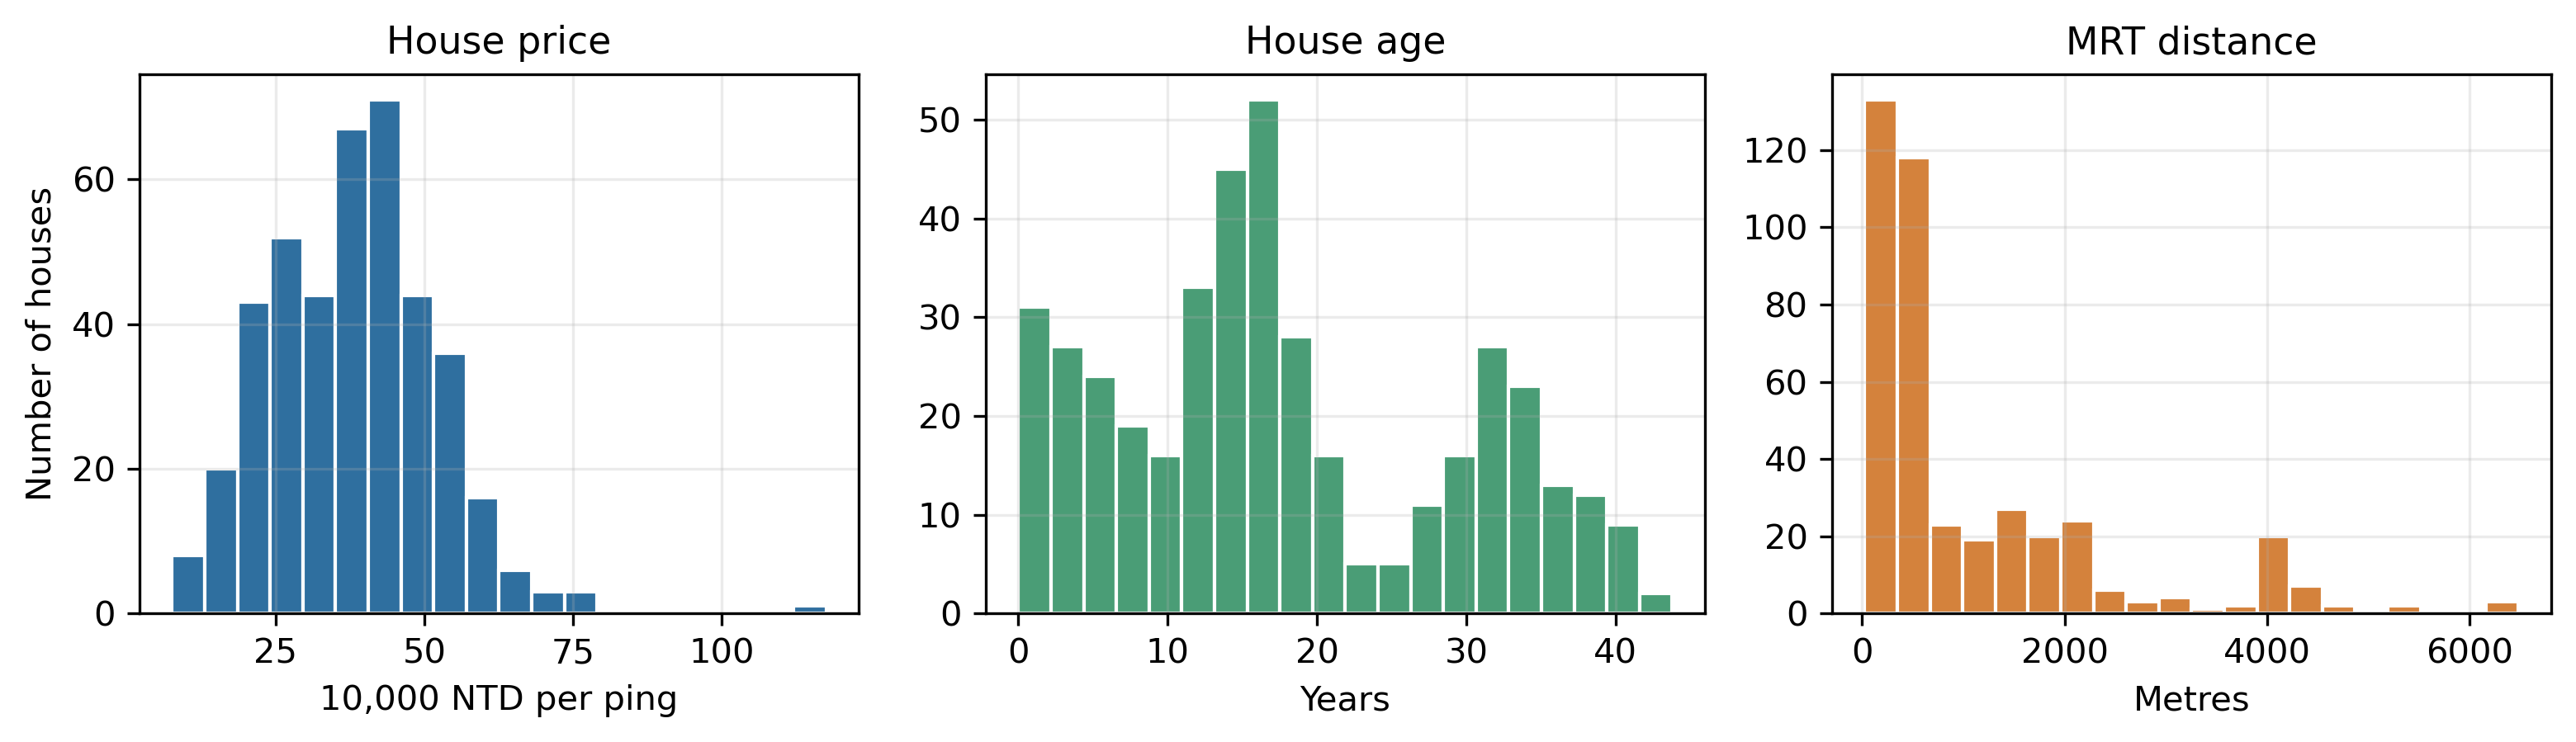
\includegraphics[width=\linewidth]{figures/eda_distributions.png}
\caption{Distributions of the target, house age, and distance to the nearest MRT
station.}
\label{fig:eda}
\end{figure}

\section{One-feature linear regression}

Using house age $x_i$ as the only feature, the prediction for house $i$ is
\begin{equation}
\hat y_i=w_0+w_1x_i.
\end{equation}
For $N$ houses, I minimized the mean squared error (MSE)
\begin{equation}
L(w_0,w_1)=\frac{1}{N}\sum_{i=1}^{N}(w_0+w_1x_i-y_i)^2.
\end{equation}
Applying the chain rule gives
\begin{align}
\frac{\partial L}{\partial w_0}
&=\frac{1}{N}\sum_i2(w_0+w_1x_i-y_i)
\frac{\partial(w_0+w_1x_i-y_i)}{\partial w_0}
=\frac{2}{N}\sum_i(w_0+w_1x_i-y_i),\\
\frac{\partial L}{\partial w_1}
&=\frac{1}{N}\sum_i2(w_0+w_1x_i-y_i)
\frac{\partial(w_0+w_1x_i-y_i)}{\partial w_1}
=\frac{2}{N}\sum_ix_i(w_0+w_1x_i-y_i).
\end{align}
Starting from $w_0=w_1=0$, I updated each parameter using
$w_j\leftarrow w_j-\eta\,\partial L/\partial w_j$. I chose
$\eta=0.001$ because it produced a smooth, stable decrease in loss, and used 20,000
epochs so the loss curve had ample time to reach a plateau.

The final values were
\begin{equation}
w_0=42.4343,\qquad w_1=-0.2515,\qquad \mathrm{MSE}=176.5005.
\end{equation}
Figure~\ref{fig:one} confirms convergence but also shows weak predictive performance.
Predictions occupy a narrow range of roughly 32--42 even though true prices range
from 7.6 to 117.5. Thus house age alone is not a strong predictor: inexpensive
houses tend to be overpredicted and expensive houses underpredicted.

\begin{figure}[H]
\centering
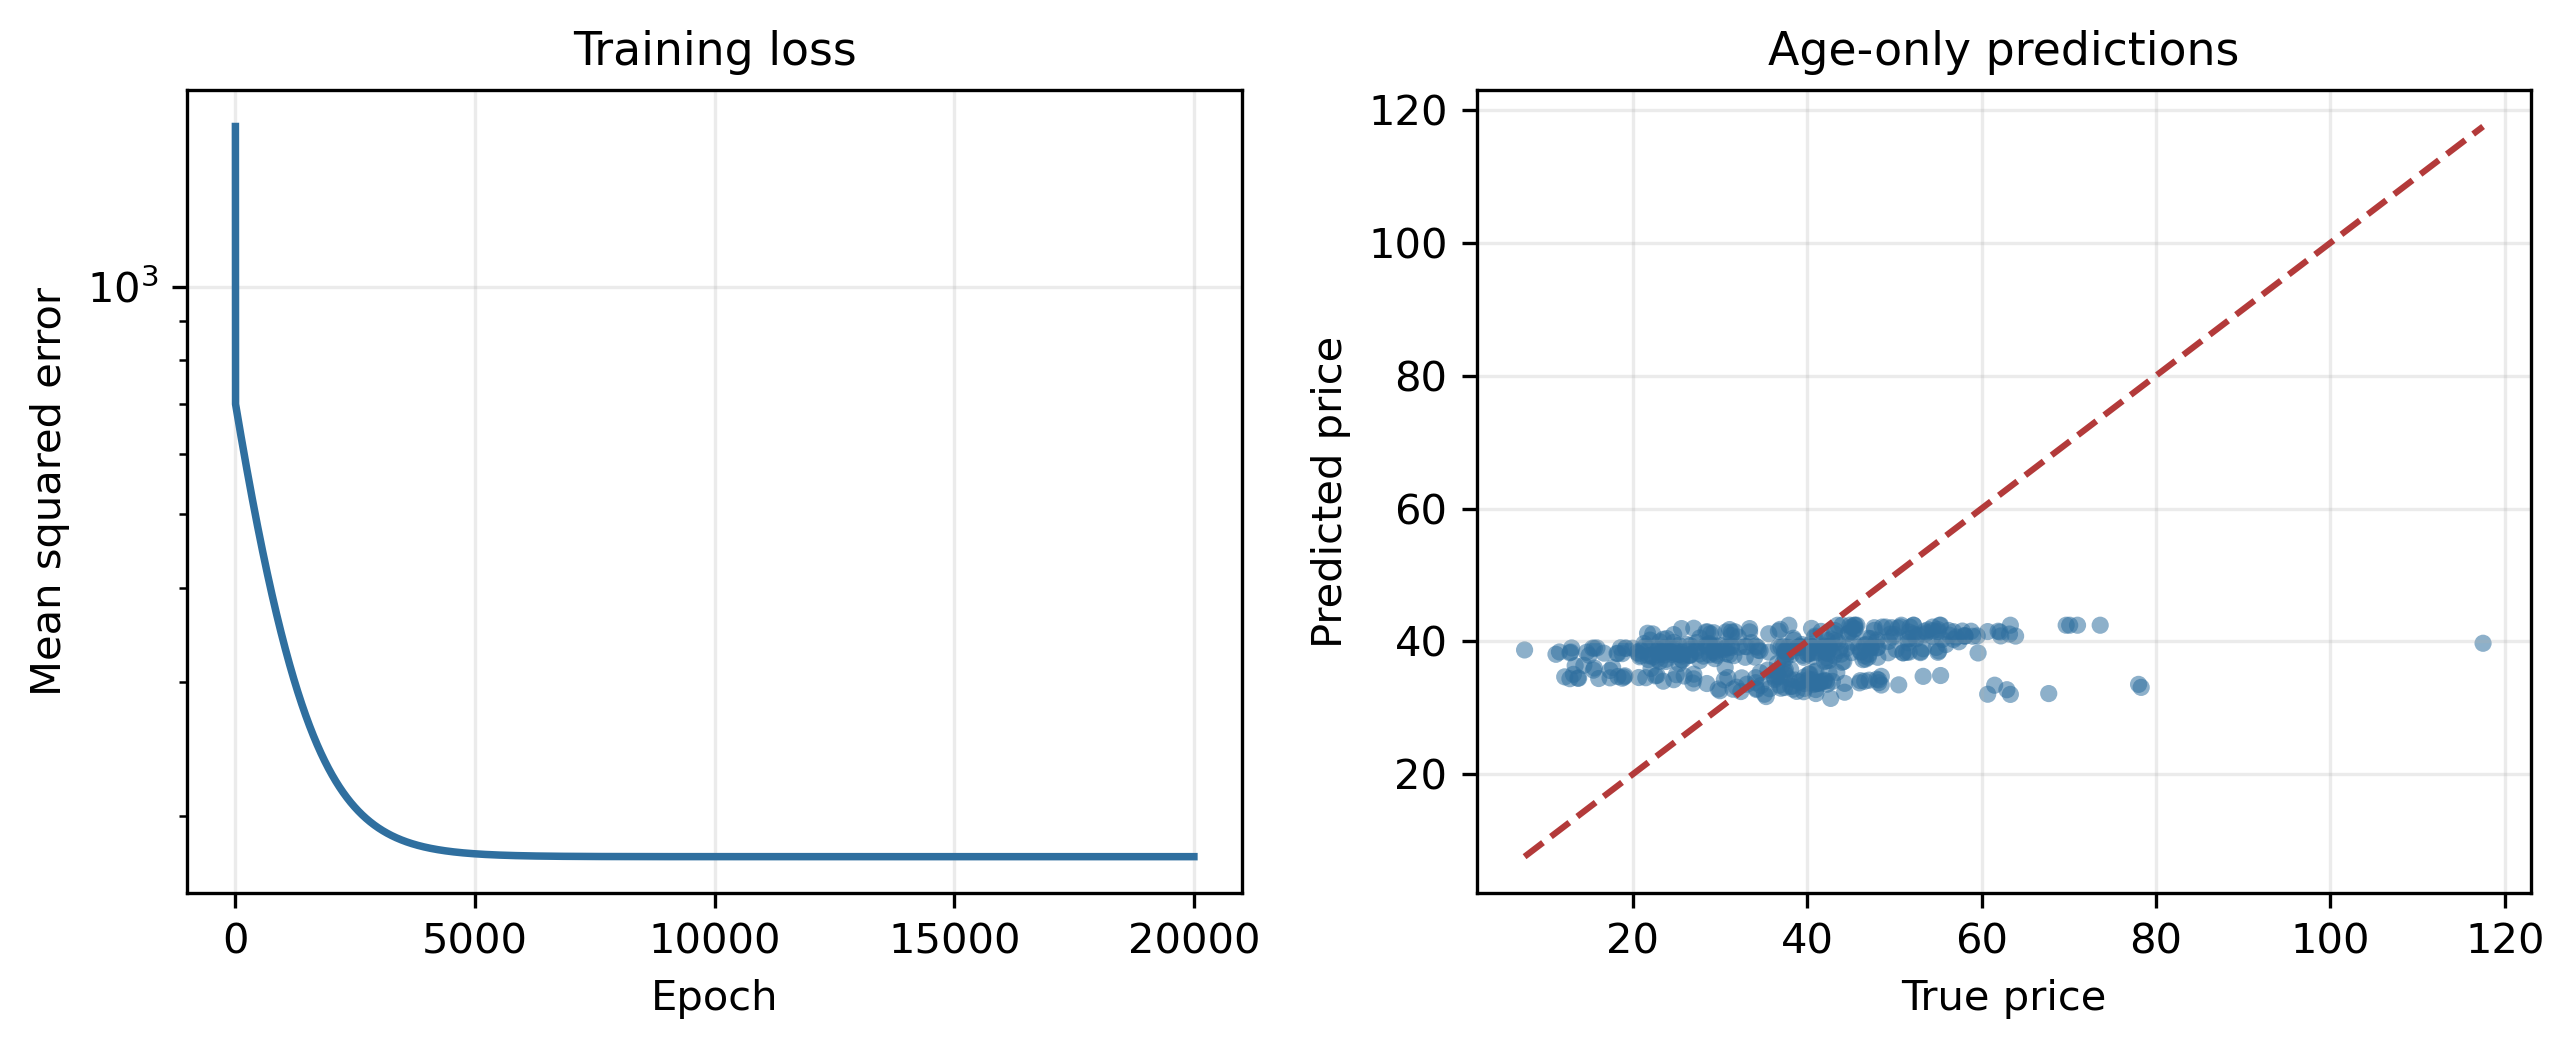
\includegraphics[width=0.92\linewidth]{figures/one_feature_results.png}
\caption{Left: MSE decreases and reaches a plateau. Right: age-only predictions
compared with the perfect-prediction line.}
\label{fig:one}
\end{figure}

\section{Multiple features and normalization}

I next used house age and distance to the nearest MRT station. With a constant 1
appended to every feature vector, the model is
\begin{equation}
\hat{\mathbf y}=X\mathbf w,
\qquad
L(\mathbf w)=\frac{1}{N}(X\mathbf w-\mathbf y)^T(X\mathbf w-\mathbf y).
\end{equation}
For weight $w_j$,
\begin{equation}
\frac{\partial L}{\partial w_j}
=\frac{2}{N}\sum_iX_{ij}(\hat y_i-y_i),
\end{equation}
so stacking all partial derivatives gives
\begin{equation}
\nabla_{\mathbf w}L=\frac{2}{N}X^T(X\mathbf w-\mathbf y),
\qquad
\mathbf w\leftarrow\mathbf w-\eta\nabla_{\mathbf w}L.
\end{equation}

Using the raw features with the same learning rate caused immediate divergence
(Fig.~\ref{fig:scaling}). MRT distances of several thousand create much larger
gradient terms than house ages of a few tens. The updates therefore overshoot the
minimum, and each subsequent update grows still larger.

I standardized each non-constant feature using
\begin{equation}
x_{\mathrm{norm}}=\frac{x-\mu_x}{\sigma_x}.
\end{equation}
This makes both feature means zero and standard deviations one. With the same
$\eta=0.001$ and 20,000-epoch limit, gradient descent converged smoothly to
\begin{equation}
\mathbf w=
\begin{bmatrix}37.9802&-2.6288&-9.0871\end{bmatrix}^{T},
\qquad \mathrm{MSE}=93.9798.
\end{equation}
Because the features are normalized, the slopes describe changes per standard
deviation. Holding the other feature fixed, a one-standard-deviation increase in
house age changes predicted price by $-2.63$, whereas the same increase in MRT
distance changes it by $-9.09$.

\begin{figure}[H]
\centering
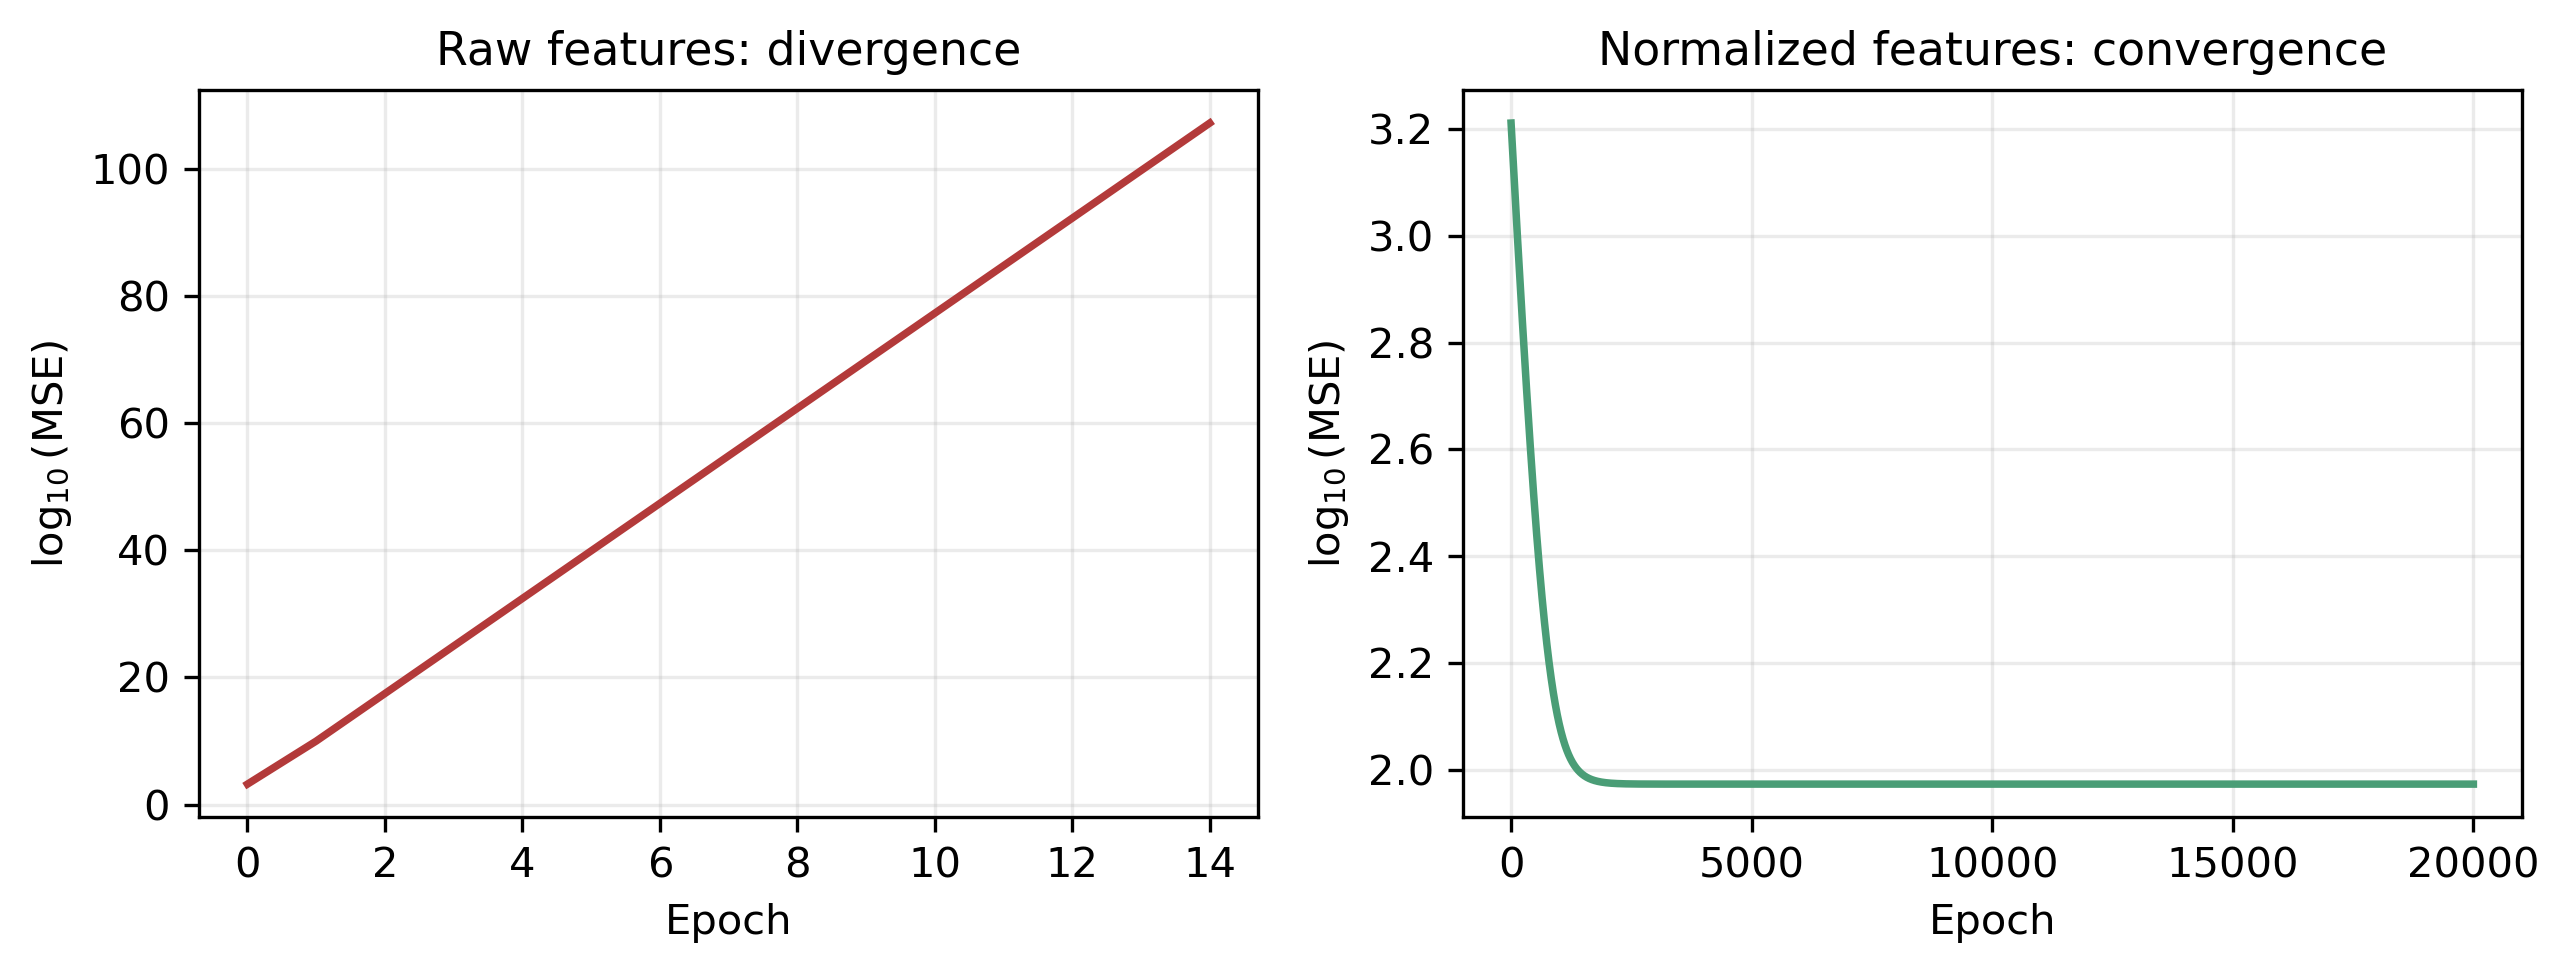
\includegraphics[width=0.92\linewidth]{figures/scaling_comparison.png}
\caption{The raw-feature loss grows explosively, while normalization gives stable
convergence with the same learning rate.}
\label{fig:scaling}
\end{figure}

\section{Model comparison and lessons}

Adding MRT distance reduced MSE from 176.50 to 93.98, a 46.8\% reduction. The
multi-feature predictions cover a wider range and generally lie closer to the
perfect-prediction line (Fig.~\ref{fig:comparison}). However, neither model captures
the most expensive observation, and the linear model still compresses predictions
toward the center of the target distribution.

\begin{figure}[H]
\centering
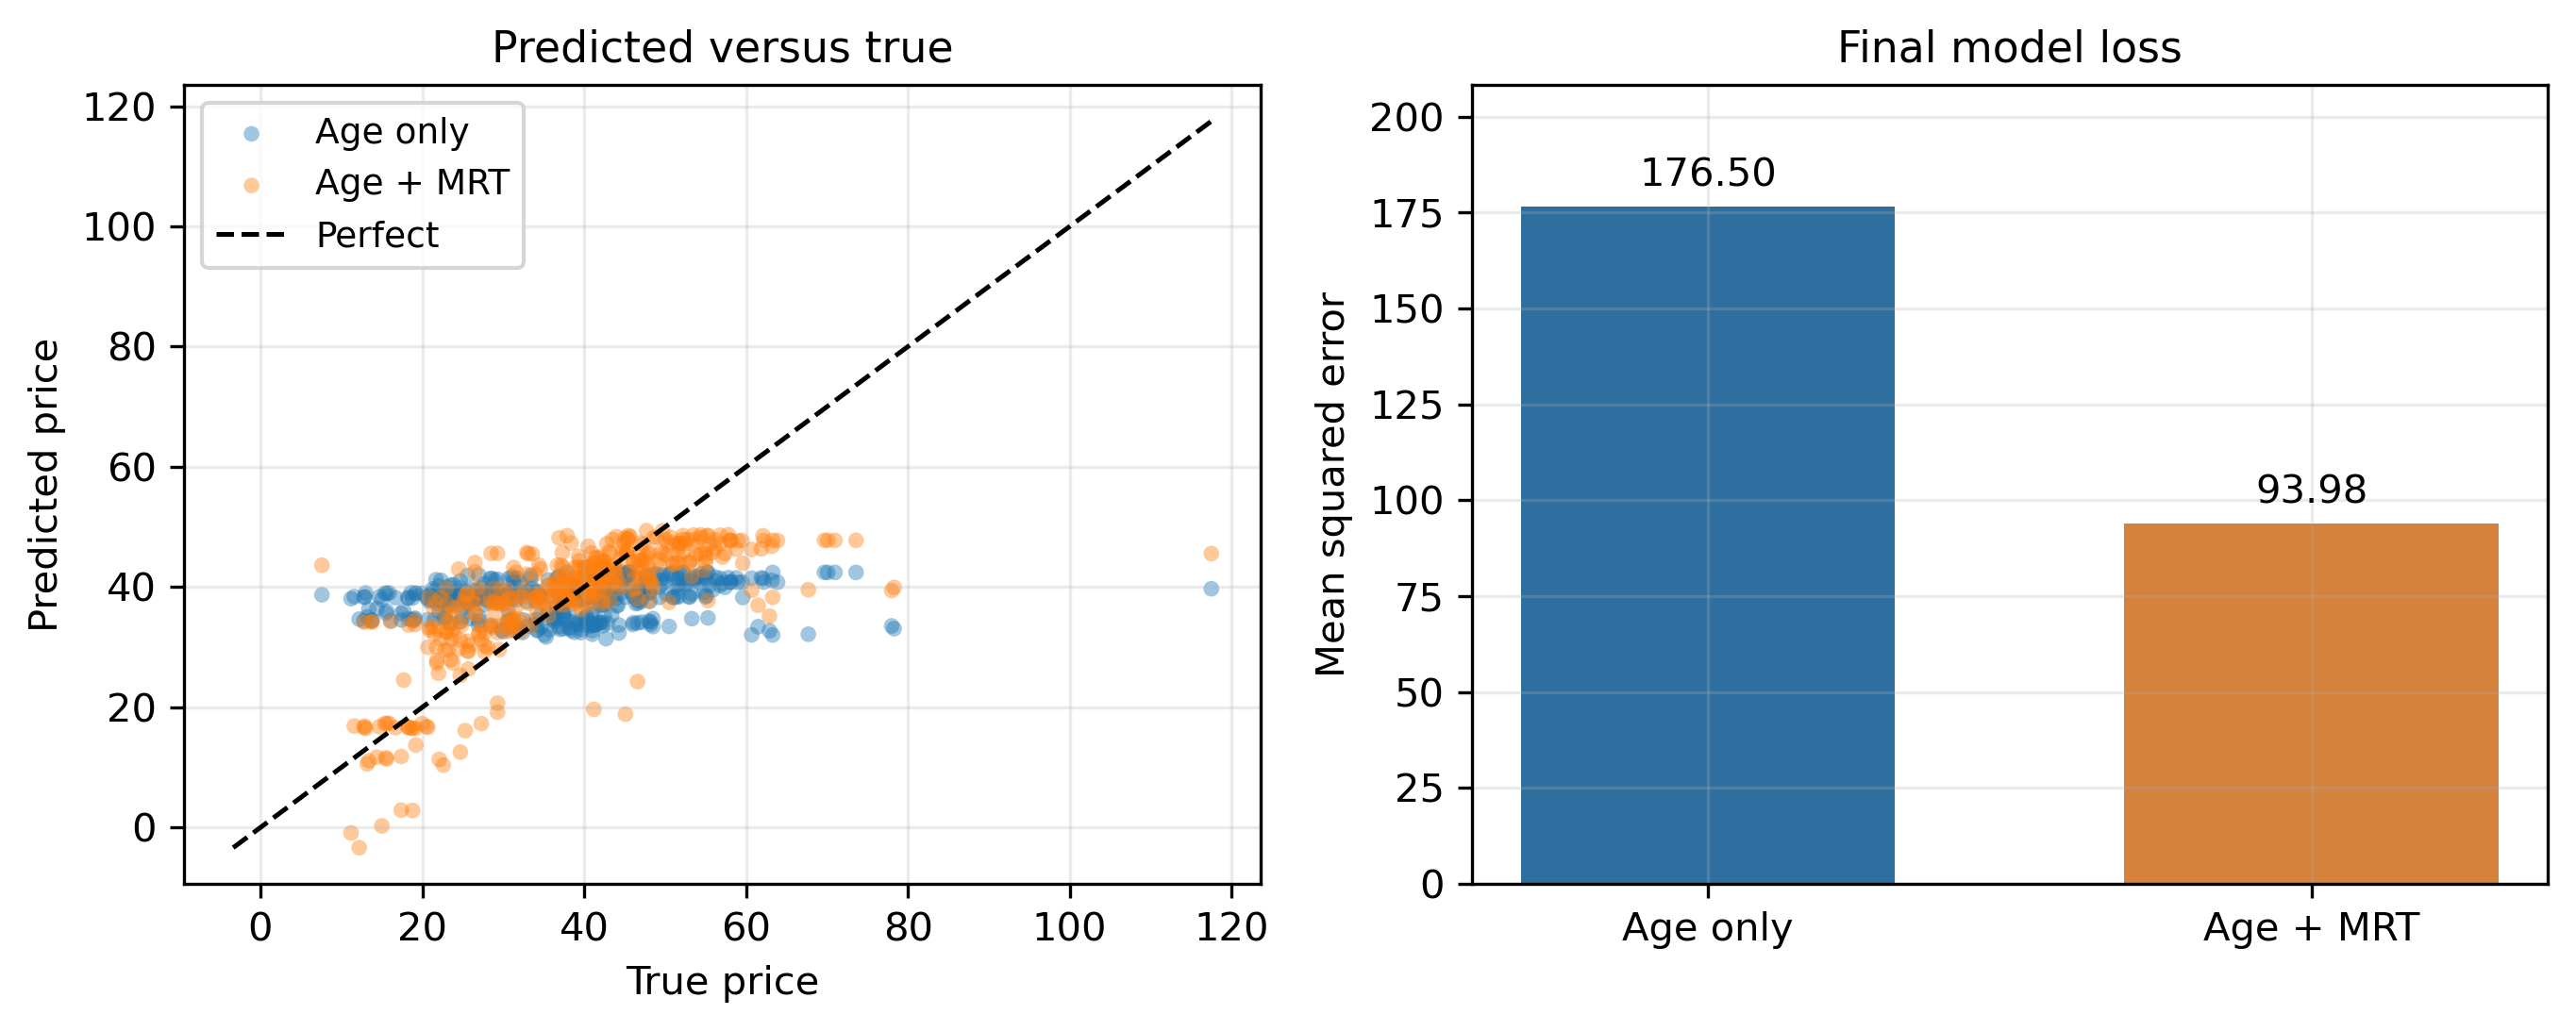
\includegraphics[width=0.94\linewidth]{figures/model_comparison.png}
\caption{Comparison of predicted-versus-true price and final MSE.}
\label{fig:comparison}
\end{figure}

The feature plots in Fig.~\ref{fig:relationships} support the numerical result.
House age contains some information, but the relationship is weak and noisy. MRT
distance carries substantially more information: prices generally decline as
distance increases. Feature scale was the main optimization limitation on the raw
data. After normalization, the learning rate was stable and the loss plateaued well
before 20,000 epochs, so the epoch count was not limiting. The extreme target near
117.5 and the restriction to a linear relationship remain important limitations.

\begin{figure}[H]
\centering
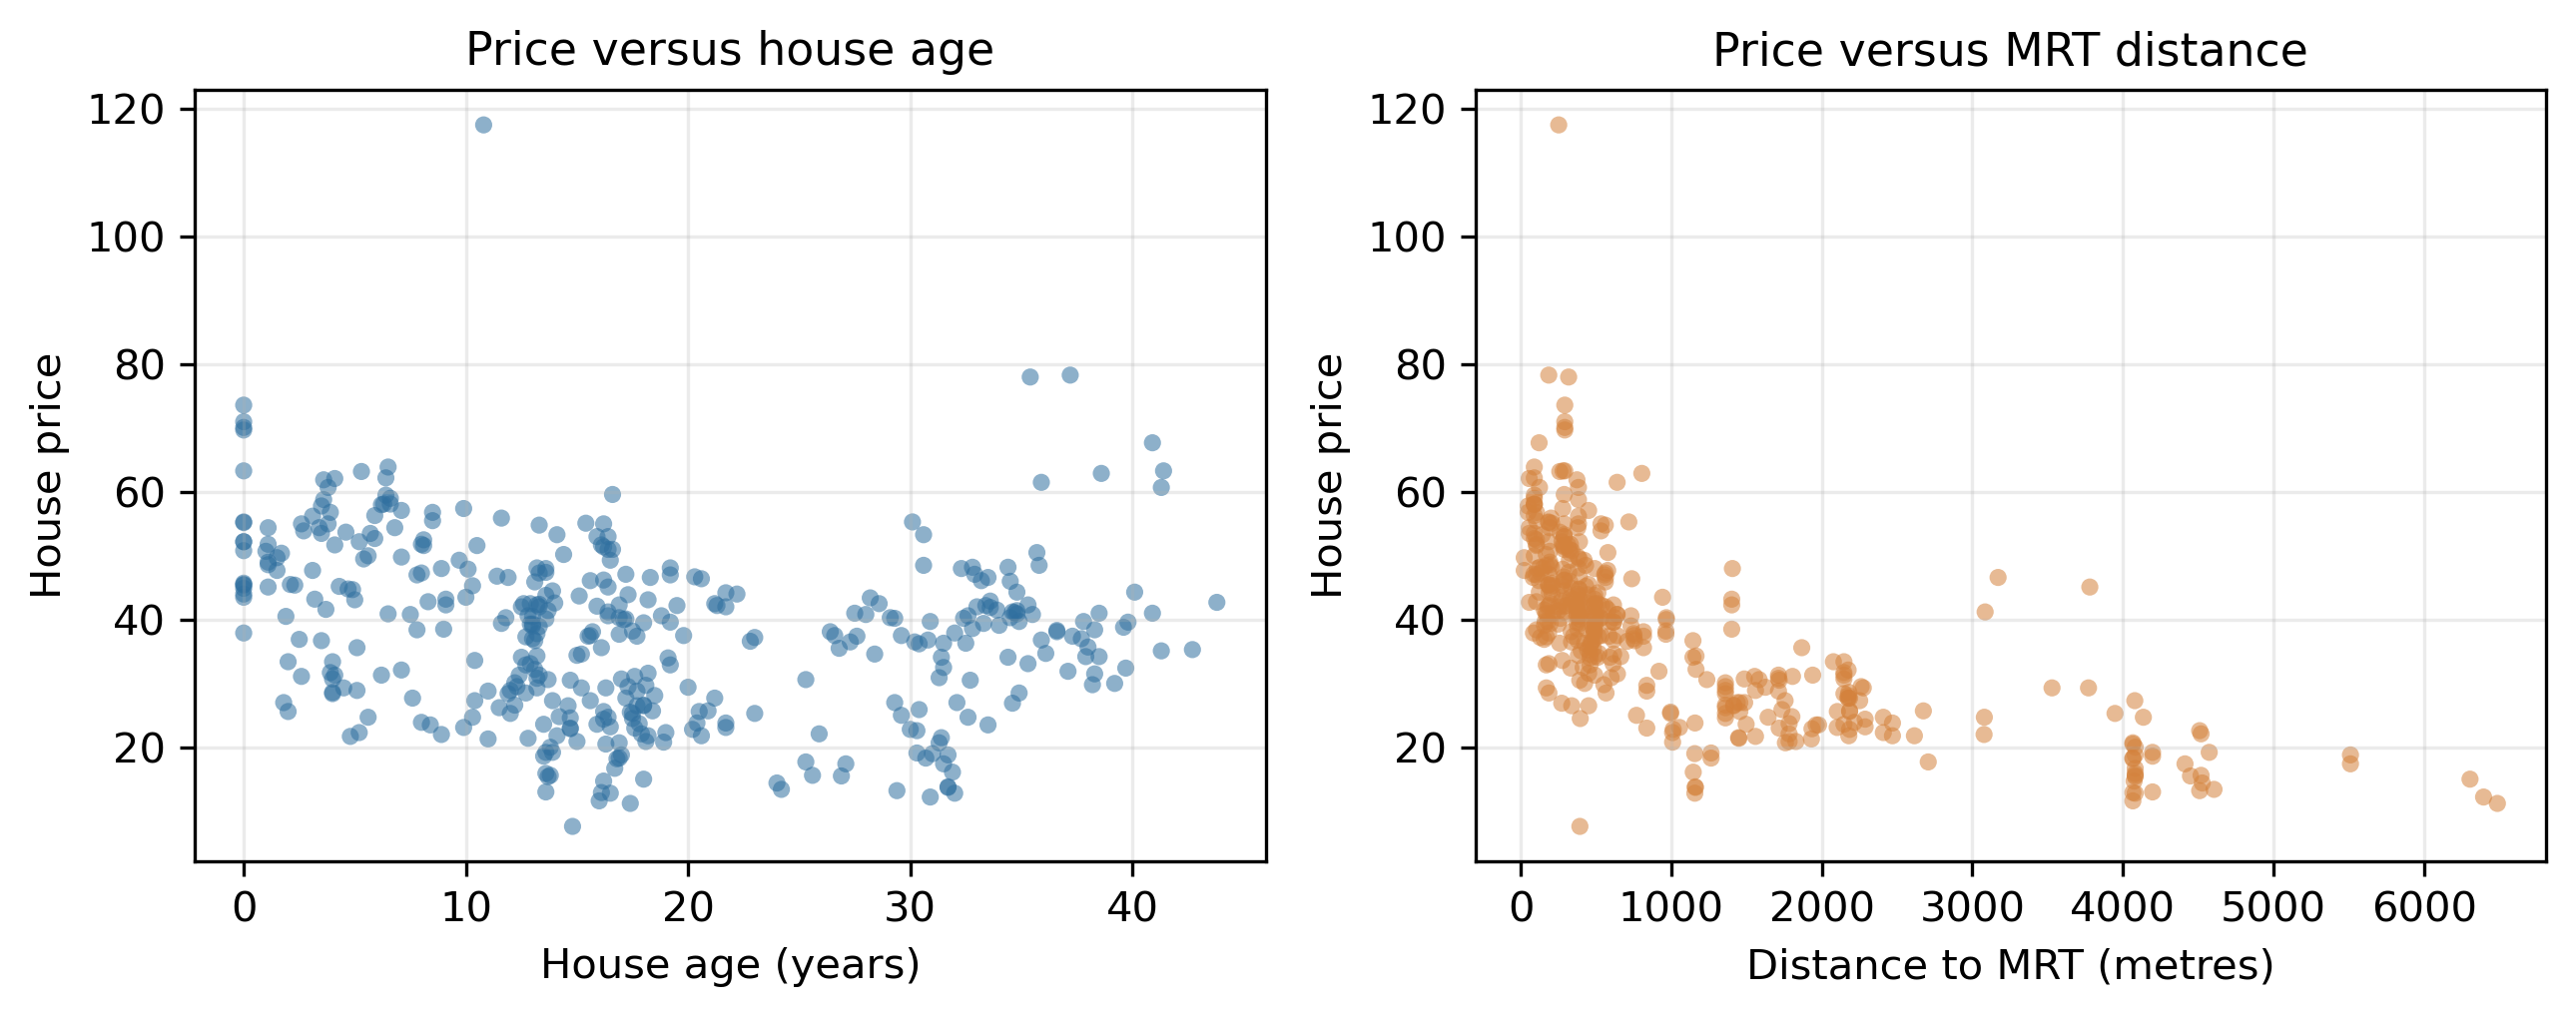
\includegraphics[width=0.92\linewidth]{figures/feature_relationships.png}
\caption{Price has a weak relationship with house age and a clearer negative
relationship with MRT distance.}
\label{fig:relationships}
\end{figure}

In a more careful version, I would investigate unusual observations, add location
and nearby-convenience-store information, and test nonlinear terms. I would also
reserve held-out data for evaluation, since the losses reported here measure fit to
the same observations used for training and do not establish performance on unseen
houses.

\section{Bonus: closed-form solution}

Setting the gradient equal to zero gives the normal equation
\begin{equation}
\mathbf w_{\mathrm{closed}}=(X^TX)^{-1}X^T\mathbf y.
\end{equation}
I solved $(X^TX)\mathbf w=X^T\mathbf y$ using
\texttt{numpy.linalg.solve}, which is mathematically equivalent but avoids explicitly
forming the inverse. The resulting weights were
$[37.9802,-2.6288,-9.0871]^T$ with MSE 93.9798. After 20,000 epochs, the largest
absolute difference between gradient-descent and closed-form weights was
$1.78\times10^{-12}$, and the loss difference was $1.42\times10^{-14}$.

I defined ``close enough'' as every weight being within 0.001 of its closed-form
value. With normalized features, this discrepancy has a negligible effect on a
typical prediction relative to the model's residual errors. Gradient descent first
met this criterion after 5,268 epochs. The agreement verifies that the implemented
gradient converges to the least-squares solution.

\begin{thebibliography}{1}
\bibitem{uci}
I.-C. Yeh, ``Real Estate Valuation,'' UCI Machine Learning Repository, 2018.
doi: \href{https://doi.org/10.24432/C5J30W}{10.24432/C5J30W}.
\end{thebibliography}

\end{document}
